\subsection{Methodology}
We propose a methodology to demystify GPU microarchitecture features and correlate them with performance. The workflow consists of three components: CUDA binary tools, a instruction solver, and deliberate microbhenchmarks. We leverage CUDA binary tools to generate disassembly codes from sample programs or libraries. A sample program is a synthetic CUDA file targeted to generate some specific instructions. A library might provide a high coverage of instruction sets. For example, the CUBLAS library contains almost all instructions used in SGEMM routines. As introduced in section~\ref{sec:cuda}, these generated assembly files ({\em sass}) provide a instruction encoded number to be cracked.

The instruction solver takes the assembly files as input to decode $64$-bits binary representation of each instruction. We design a set of algorithms to solve all fields of the binary instruction. These fields include various {\em operands}, {\em opcodes} and {\em modifiers}. The solver retrieves the undocumented ISA specification, which is used to implement an native assembler. Then, we design deliberate microbenchmarks and leverage the assembler to tune code at assembly language level. In the end, the tuning process will lead to some practical observations on the correlation between microarchitecture and performance.

\begin{figure}[htbp]
\begin{center}
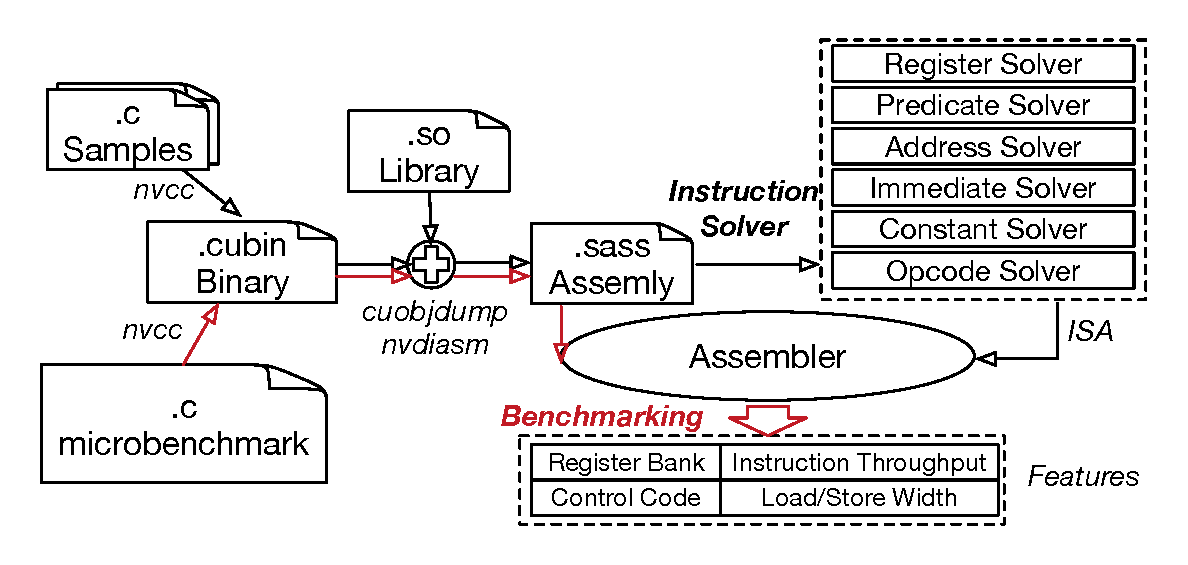
\includegraphics[scale=0.45]{methodology}
\caption{A schematic diagram of demystifying GPU microarchitecture features by leveraging CUDA binary tools. The black arrows represent the workflow of instruction solver while the red ones represents benchmarking to find out correlation between microarchitecture and performance.}
\label{fig:workflow}
\end{center}
\end{figure}


